% Optional manuscript block. Requires booktabs and graphicx.
% Paths assume compilation from the repository root.
% Numerical text describes the current full saved run; recheck if models/data change.
\subsection{Parameter estimation and goodness of fit}
\label{sec:parameter-estimation-results}

The proposed model was fitted to 147 standardized-meal windows from
30 participants, using 4,452 post-meal CGM observations, including meal
time. Participant-level kinetic parameters were shared across that
participant's retained meals, while meal amplitude and absorption delay
were event-specific. All fitted participants and events were retained in
the performance summaries, including poorly fitted trajectories.
These results describe in-sample reconstruction; no independent
test cohort or held-out meal evaluation is used here.

Table~\ref{tab:fit-overall} reports two complementary summaries of error:
pooled RMSE and MAE across observed time points, and the distribution of
participant-level errors, giving each participant equal weight.
The proposed model achieved a pooled RMSE of 10.83~mg/dL and MAE of
7.00~mg/dL, compared with 11.26 and 7.33~mg/dL for the reduced two-state
model. Median participant RMSE was 9.14~mg/dL [Q1, Q3: 7.72, 10.97].
The proposed model had lower RMSE for 22 of 30 participants, but lower
nominal BIC for only 14 of 30. Thus, its lower aggregate reconstruction
error does not establish a uniform advantage after accounting for
model complexity.

To avoid attributing between-meal starting-glucose differences to
successful reconstruction of meal-response dynamics, we additionally
report a within-event coefficient of determination,
\[
R^2_{\mathrm{within}}
=1-\frac{\sum_e\sum_t(G_{et}-\widehat G_{et})^2}
             {\sum_e\sum_t(G_{et}-\bar G_e)^2},
\]
where $\bar G_e$ is the observed mean for event $e$. Its value was 0.665
for the proposed model and 0.638 for the reduced model. The median
event-level $R^2$ was 0.615 [0.287, 0.853] for the proposed model, and
22 of 147 events had negative $R^2$, indicating greater squared error
than a constant predictor equal to that event's observed mean.
Meal-time observations inform initial conditions; these fit scores
must not be interpreted as prospective prediction accuracy.

% Requires booktabs and graphicx.
\begin{table}[htbp]
\centering
\caption{Overall in-sample goodness of fit across all fitted participants and meals.}
\label{tab:fit-overall}
\small
\resizebox{\linewidth}{!}{%
\begin{tabular}{lrr}
\toprule
Outcome & Proposed 3-state & Reduced 2-state \\
\midrule
Participants & 30 & 30 \\
Meal windows & 147 & 147 \\
CGM observations & 4,452 & 4,452 \\
Pooled RMSE (mg/dL) & 10.83 & 11.26 \\
Pooled MAE (mg/dL) & 7.00 & 7.33 \\
Participant RMSE, median [Q1, Q3] & 9.14 [7.72, 10.97] & 9.71 [7.88, 11.38] \\
Participant MAE, median [Q1, Q3] & 6.53 [5.17, 7.65] & 7.35 [5.21, 7.85] \\
Within-event $R^2$ & 0.665 & 0.638 \\
Event $R^2$, median [Q1, Q3] & 0.615 [0.287, 0.853] & 0.612 [0.280, 0.819] \\
Events with $R^2$ $<$ 0 & 22/147 & 24/147 \\
Lower participant RMSE & 22/30 & 8/30 \\
Lower nominal AIC & 17/30 & 13/30 \\
Lower nominal BIC & 14/30 & 16/30 \\
\bottomrule
\end{tabular}}
\par\smallskip
\begin{minipage}{\linewidth}\footnotesize
All fitted participants and meal windows are included, with no outcome-based exclusions. Errors are unweighted and in-sample at the observed times ($t\geq0$); the meal-time observation also informs model initialization. Pooled RMSE and MAE weight observations equally; participant summaries weight people equally. Within-event $R^2=1-\sum_e\mathrm{SSE}_e/\sum_e\sum_t(G_{et}-\bar G_e)^2$, which removes between-event baseline differences. Event summaries include negative $R^2$ values; constant-glucose events have undefined $R^2$. Q1 and Q3 are quartiles, not confidence bounds. Lower-metric counts compare the two models within each participant. AIC/BIC are nominal residual-based criteria from the original fit, without a serial-correlation correction. These are training fits, not held-out validation.
\end{minipage}
\end{table}


Figure~\ref{fig:selected-model-fits} illustrates well-reconstructed
responses, selecting the event with the highest proposed-model $R^2$
within each clinical-status group. This deliberately favorable selection
is used only to illustrate fitted trajectory shapes, not to estimate
typical cohort performance. Figure~\ref{fig:fit-cohort-diagnostics} and
Table~\ref{tab:fit-overall} retain all fitted cases.

\begin{figure*}[t]
\centering
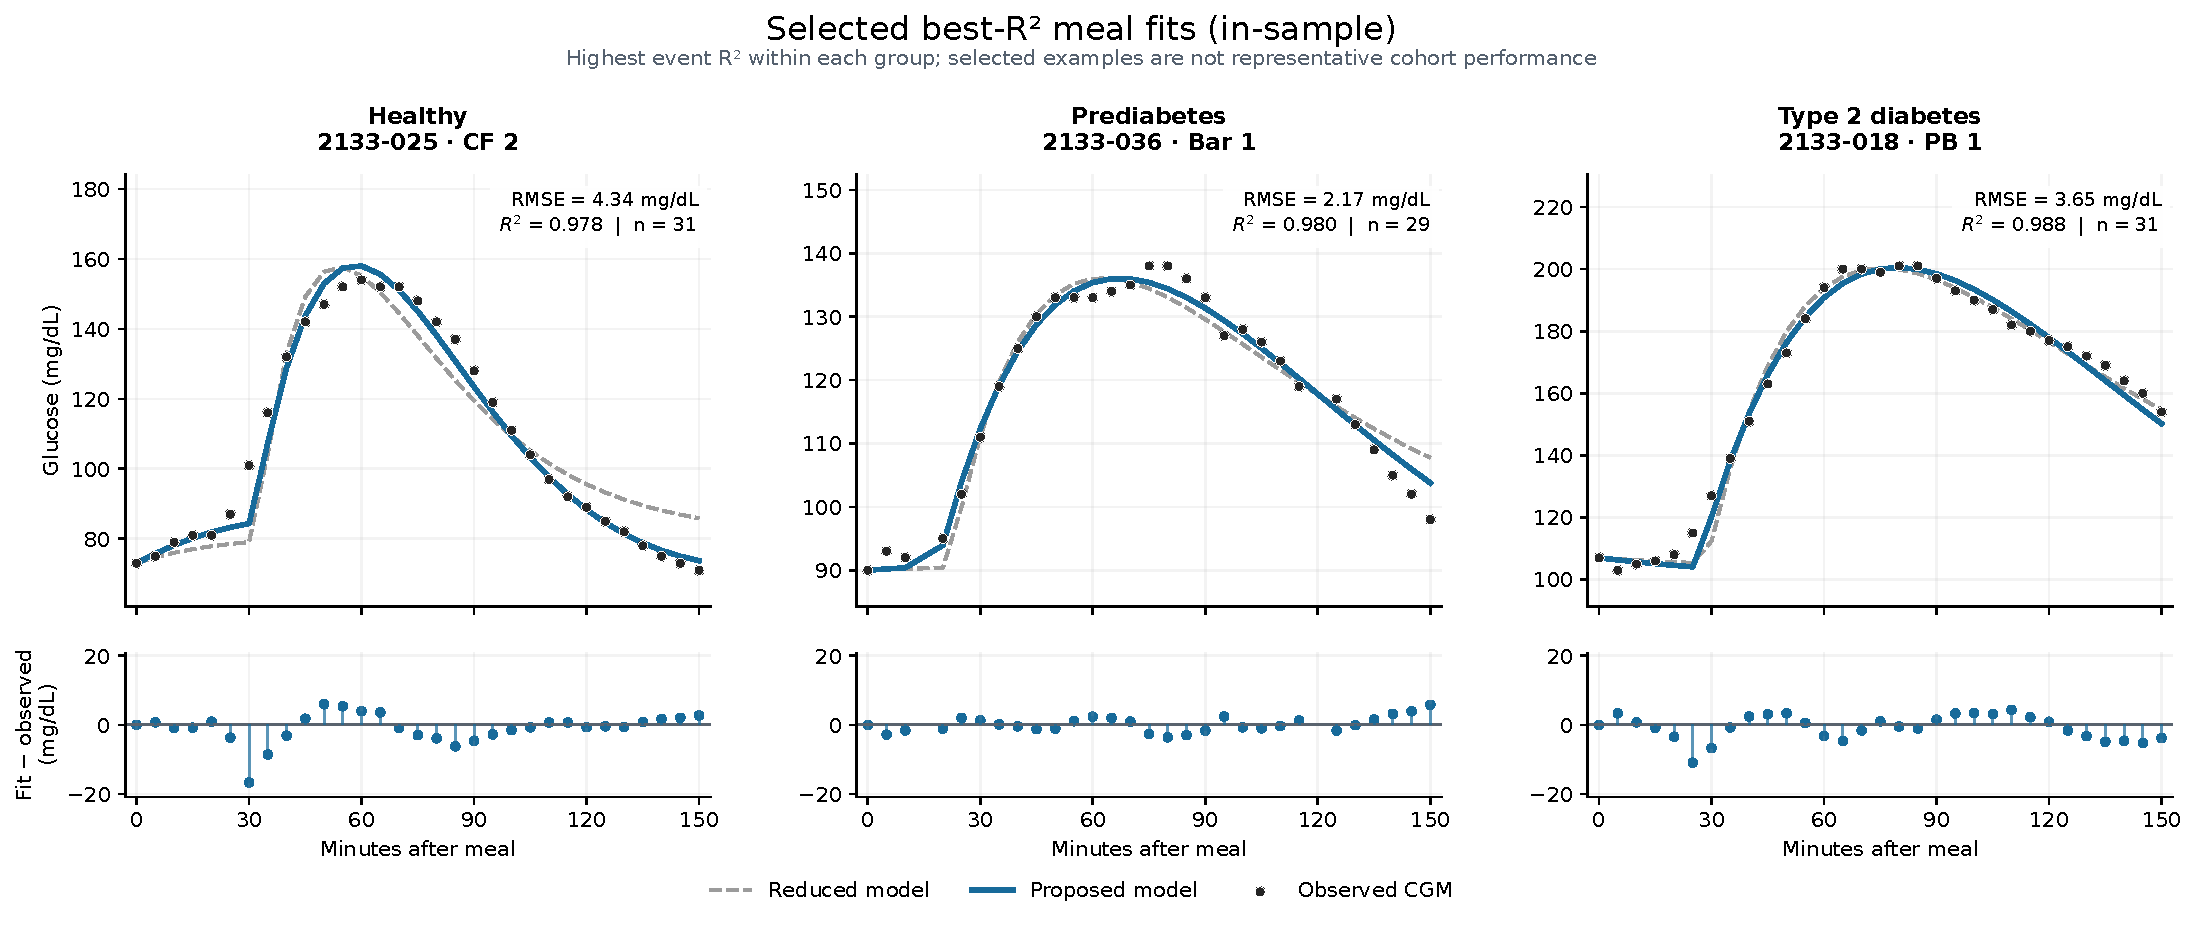
\includegraphics[width=\textwidth]{outputs/figures/figure_3_selected_model_fits.pdf}
\caption{Selected high-$R^2$ in-sample meal fits. One event is selected
within each clinical-status group by maximum proposed-model event
$R^2$, with ties resolved by lower RMSE and then event identifier.
The selected events are 2133-025/CF~2 (Healthy), 2133-036/Bar~1
(prediabetes), and 2133-018/PB~1 (type 2 diabetes).
Black points show every available fitted CGM observation in the selected
event; blue lines connect saved proposed-model predictions and dashed
gray lines connect reduced-model predictions at those observation times.
No measured points are removed or smoothed for display. Bottom panels
show proposed-model residuals (fitted minus observed glucose) on a shared
vertical scale. Upper-panel glucose axes have different ranges.
Each event uses participant parameters estimated jointly from all that
person's fitted meals, not a separate refit of the selected event.
These selected examples are not representative estimates of cohort
performance and do not constitute out-of-sample validation.}
\label{fig:selected-model-fits}
\end{figure*}

\begin{figure*}[t]
\centering
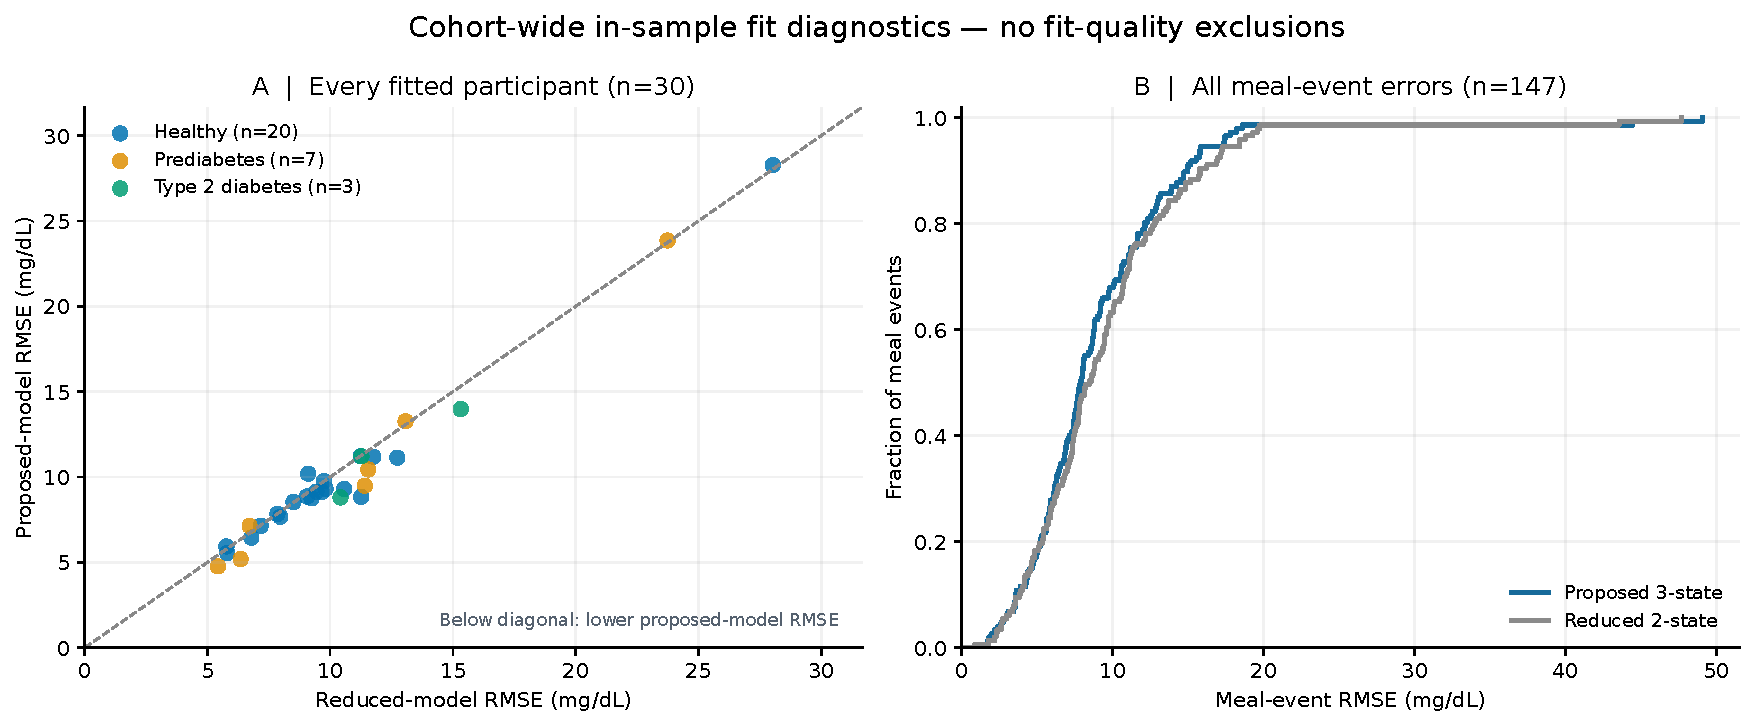
\includegraphics[width=\textwidth]{outputs/figures/figure_7_fit_diagnostics.pdf}
\caption{Cohort-wide goodness-of-fit diagnostics without fit-quality
exclusions. (A) Paired participant RMSE for all 30 fitted participants;
points below the identity line have lower error under the proposed
model. (B) Empirical cumulative distributions of meal-event RMSE across
all 147 events for both models. A larger cumulative fraction at a given
error threshold indicates more events below that threshold. Repeated
meal events are nested within participants; no independence-based
significance claim is made. All errors are in-sample.}
\label{fig:fit-cohort-diagnostics}
\end{figure*}

Table~\ref{tab:parameter-group-comparison} compares participant-level
kinetic estimates in the Healthy ($n=20$), prediabetes ($n=7$), and
type 2 diabetes ($n=3$) groups. Prediabetes is not combined with
type 2 diabetes for the Healthy--T2D contrast. Medians and interquartile
ranges are used to describe the skewed and boundary-concentrated
estimates. For example, the median $\beta_1$ estimate is 0.526 in the
Healthy group and 0.195 in the T2D group, while the corresponding
$\delta$ medians are 2.91 and 1.40. These are descriptive differences
between fitted model parameters, not established physiological effects.

% Requires booktabs and graphicx.
\begin{table}[htbp]
\centering
\caption{Participant-level kinetic estimates by clinical status (Healthy: n=20, Prediabetes: n=7, Type 2 diabetes: n=3).}
\label{tab:parameter-group-comparison}
\small
\resizebox{\linewidth}{!}{%
\begin{tabular}{lrrrr}
\toprule
Parameter & Healthy & Prediabetes & Type 2 diabetes & T2D - Healthy median \\
\midrule
$\alpha$ & 2.79 [0.899, 4.65] & 1.3 [0.654, 1.75] & 1.49 [1.25, 3.31] & -1.3 \\
$\beta_0$ & 0.0001 [0.0001, 0.016] & 0.0001 [0.0001, 0.000101] & 0.000105 [0.000103, 0.0117] & +4.54e-06 \\
$\beta_1$ & 0.526 [0.43, 0.742] & 0.228 [0.152, 0.364] & 0.195 [0.132, 0.345] & -0.331 \\
$\beta_2$ (derived) & 470 [260, 608] & 386 [298, 556] & 704 [485, 751] & +234 \\
$\gamma$ & 9.99 [9.82, 10] & 10 [9.8, 10] & 10 [9.64, 10] & +0.00493 \\
$\delta$ & 2.91 [1.38, 6.82] & 1.79 [0.968, 1.94] & 1.4 [0.936, 3.2] & -1.52 \\
\bottomrule
\end{tabular}}
\par\smallskip
\begin{minipage}{\linewidth}\footnotesize
Entries are participant-level medians [Q1, Q3], not confidence intervals. The final column is the T2D median minus the Healthy median; prediabetes is not pooled with T2D. $\beta_2$ is derived from the equilibrium constraint, not independently fitted. Time is measured in hours; $\alpha,\beta_0,\delta$ have units h$^{-1}$; $\beta_1$ has units (model insulin unit $\times$ h)$^{-1}$; $\gamma$ has units model insulin unit/h; and $\beta_2$ has units mg/dL/h under the dimensionless-insulin convention. Insulin is not calibrated to clinical units. Small subgroup sizes and frequent boundary estimates limit interpretation; see the boundary-diagnostic table. Differences are descriptive, not hypothesis tests or proof of physiological differences; no p-values are claimed.
\end{minipage}
\end{table}

% Requires booktabs and graphicx.
\begin{table}[htbp]
\centering
\caption{Boundary diagnostics for participant-level kinetic estimates.}
\label{tab:parameter-bound-diagnostics}
\small
\resizebox{\linewidth}{!}{%
\begin{tabular}{lrrrr}
\toprule
Parameter & Search interval & Healthy & Prediabetes & Type 2 diabetes \\
\midrule
$\alpha$ & [0.05, 10] & 0/1 of 20 & 0/0 of 7 & 0/0 of 3 \\
$\beta_0$ & [0.0001, 2] & 15/0 of 20 & 7/0 of 7 & 2/0 of 3 \\
$\beta_1$ & [1e-06, 1] & 0/2 of 20 & 0/0 of 7 & 0/0 of 3 \\
$\beta_2$ (derived) & Derived & -- & -- & -- \\
$\gamma$ & [0.001, 10] & 0/14 of 20 & 0/5 of 7 & 0/2 of 3 \\
$\delta$ & [0.05, 10] & 0/1 of 20 & 0/0 of 7 & 0/0 of 3 \\
\bottomrule
\end{tabular}}
\par\smallskip
\begin{minipage}{\linewidth}\footnotesize
Entries are lower/upper boundary counts out of the group size. A value is near a bound when its distance is less than 0.5\% of the full search-interval width, matching the fitting pipeline. These counts denote proximity, not necessarily exact optimizer contact. The equilibrium-derived $\beta_2$ has no independently optimized search interval.
\end{minipage}
\end{table}


Boundary and identifiability diagnostics are essential to interpreting
these comparisons. Twenty-eight of 30 participants have at least one
kinetic estimate within 0.5\% of a search-interval boundary. In particular,
$\beta_0$ is near its lower bound in 24 fits, and $\gamma$ is near its
upper bound in 21 fits. All 30 normalized kinetic-Jacobian condition
numbers exceed 100. Moreover, $\beta_2$ is derived from an equilibrium
constraint rather than estimated independently, and insulin is latent
and uncalibrated to clinical units. Together with the small T2D subgroup,
these features limit mechanistic interpretation. The tables therefore
make descriptive comparisons without claims of statistical significance,
disease-specific parameter identification, or clinical validity.
